\part{Simulation}
\frame{\partpage}

\begin{frame}{What is simulation?}
	\begin{itemize}
		\pause\item Replicating (physical) behaviour using equations (e.g. Newton's Laws of Motion).
		\pause\item Different kinds of objects behave differently:
		\begin{itemize}
			\pause\item Motion through space resulting from external forces - \textbf{particle simulation}
			\pause\item Changes in orientation resulting from external forces - \textbf{rigid body dynamics}
			\pause\item Changes in shape resulting from external \textit{and internal} forces - \textbf{soft-body deformation}
			\begin{itemize}
				\pause\item Some types of object have specific techniques, e.g. \textbf{hair, cloth} and \textbf{fluid}
			\end{itemize}
			\pause\item Automating aspects of manual animation processes - e.g. \textbf{inverse kinematics (IK)}
		\end{itemize}
	\end{itemize}
\end{frame}

\begin{frame}{Particle simulation}
	\begin{columns}
		\begin{column}{0.3\textwidth}
			\begin{figure}
				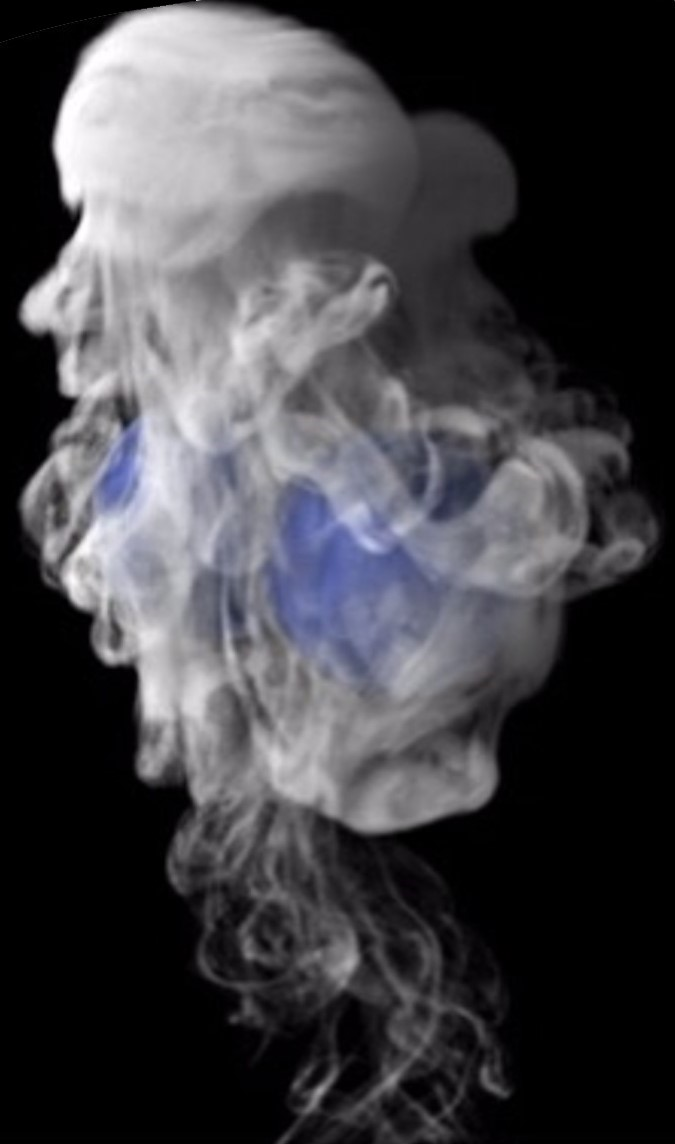
\includegraphics[width=\textwidth]{particles}
				\caption*{Image courtesy of \href{https://www.framestore.com}{Framestore}}
			\end{figure}
		\end{column}
		\begin{column}{0.65\textwidth}
			\begin{itemize}
				\pause\item Used to predict the behaviour of dimensionless \textbf{point mass} objects
				\pause\item Computed one frame at a time, to account for \textbf{collisions}
				\pause\item Can be used for fluid-like effects such as smoke
			\end{itemize}
		\end{column}
	\end{columns}
\end{frame}

\begin{frame}{Rigid body dynamics}
	\begin{columns}
		\begin{column}{0.3\textwidth}
			\begin{figure}
				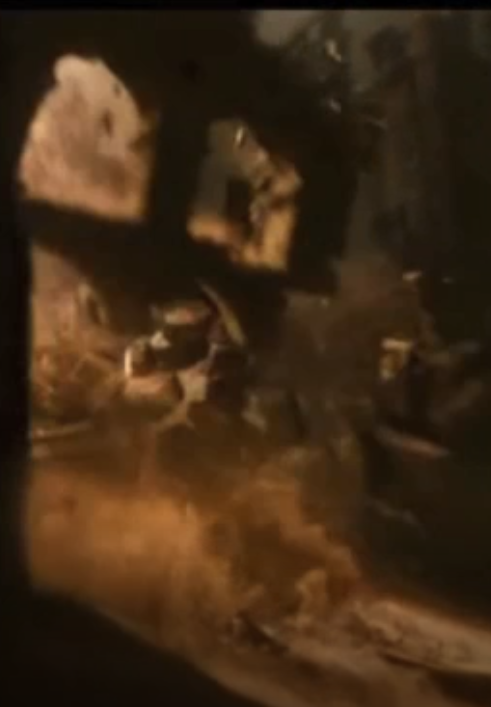
\includegraphics[width=\textwidth]{rigid_bodies}
				\caption*{Image courtesy of \href{https://www.framestore.com}{Framestore}}
			\end{figure}
		\end{column}
		\begin{column}{0.65\textwidth}
			\begin{itemize}
				\pause\item Used to predict the behaviour of \textbf{non-deformable} objects
				\pause\item Global motion is computed as for particles...
				\pause\item ... combined with local motion (rotation) about the object's centre of mass
				\pause\item Commonly used for destruction sequences
			\end{itemize}
		\end{column}
	\end{columns}
\end{frame}

\begin{frame}{Soft body dynamics}
	\begin{columns}
		\begin{column}{0.3\textwidth}
			\begin{figure}
				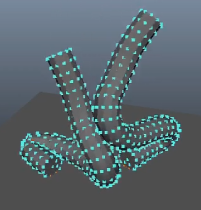
\includegraphics[width=\textwidth]{soft_bodies}
				\caption*{Image courtesy of \href{https://www.framestore.com}{Framestore}}
			\end{figure}
		\end{column}
		\begin{column}{0.65\textwidth}
			\begin{itemize}
				\pause\item Used to predict the behaviour of \textbf{deformable} objects
				\pause\item Requires knowledge of the interior of an object (e.g. FEM): computationally very expensive
				\pause\item Often approximated using \textbf{constrained rigid bodies} and other techniques
			\end{itemize}
		\end{column}
	\end{columns}
\end{frame}

\begin{frame}{Other types of dynamic simulation}
	\begin{columns}
		\begin{column}{0.3\textwidth}
			\begin{figure}
				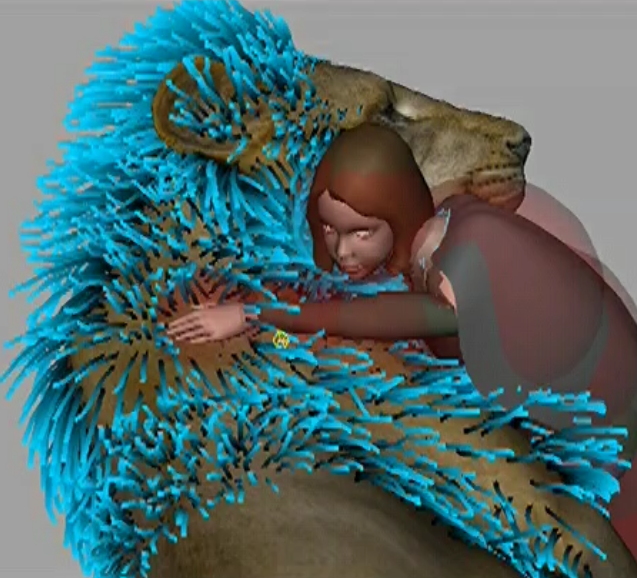
\includegraphics[width=\textwidth]{hair}
				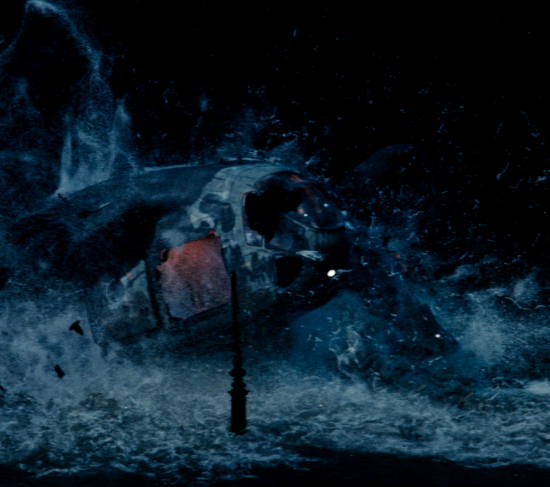
\includegraphics[width=\textwidth]{fluid}
				\caption*{Images courtesy of \href{https://www.framestore.com}{Framestore}}
			\end{figure}
		\end{column}
		\begin{column}{0.65\textwidth}
			\begin{itemize}
				\pause\item Objects such as \textbf{hair, cloth} and \textbf{liquids} behave slightly differently
				\pause\item These have their own equations and techniques...
				\pause\item Beyond the scope of this module!
			\end{itemize}
		\end{column}
	\end{columns}
\end{frame}

\begin{frame}{Rigging and animation}
	\begin{columns}
		\begin{column}{0.3\textwidth}
			\begin{figure}
				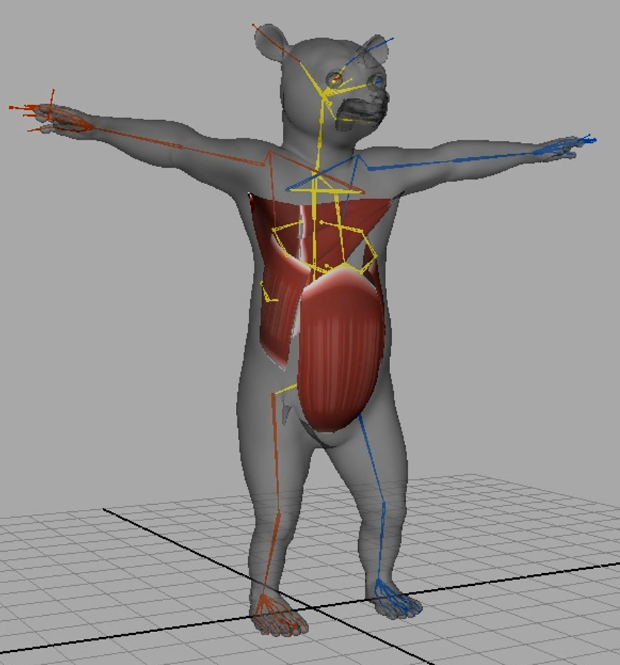
\includegraphics[width=\textwidth]{rigging}
				\caption*{Image courtesy of \href{https://www.framestore.com}{Framestore}}
			\end{figure}
		\end{column}
		\begin{column}{0.65\textwidth}
			\begin{itemize}
				\pause\item Key characters (and objects) are hand-animated by artists using a \textbf{skeleton rig}
				\pause\item Positioning each joint would be a laborious process...
				\pause\item Techniques such as Inverse Kinematics (IK) have been developed to automate certain aspects.
			\end{itemize}
		\end{column}
	\end{columns}
\end{frame}